%!TEX root = ../var.tex

\begin{definition} 
\label{def:5.1}
События A и B называются \textit{независимыми}, если выполняется тождество
\begin{equation*}
	\P(A \cap B) = \P(A)\P(B),
\end{equation*}
в противном случае они называются \textit{зависимыми}.
\end{definition}
	
\textbf{Примеры}. 

1) Рассмотрим колоду карт в 52 листа. 
Пусть событие $A$ означает вытянуть пику $\spadesuit$, а $B$ означает вытянуть даму \textbf{Д}, Тогда событие $A\cap B$ означает вытянуть пиковую даму \textbf{Д$\spadesuit$}. Легко подсчитать вероятности этих событий $\P(A\cap B)$ = 1/52; $\P(A) = 1/4$ и $\P(B) = 1/13$. Подставив эти вероятности в равенство опред. \ref{def:5.1}, получим тождество $1/52 = 1/4 \cdot1/13$; т.е. по опред. \ref{def:5.1} события $A$ и $ B $ независимы (в этой колоде).


2) Рассмотрим полную колоду карт в 54 листа (с двумя шутами). 
Пусть события $A$ и $B$ — те же как в предыдущем пункте. 
Легко подсчитать, что в этой колоде $\P(A \cap B) = 1/54$, $\P(A) = 13/54$ и $\P(B) = 2/27$. 
Таким образом $1/54 \neq 13/54 \cdot 2/27$, и по опред. \ref{def:5.1} события $A$ и $B$ являются зависимыми в полной колоде. 
Получилось, что свойство быть или не быть независимыми зависит не от самих событий, а от строения пространства $\Omega$ (52 или 54).

\begin{lemma}
\label{lemma:5.2}
Если события $A$ и $B$ независимы, то пары событий $A$ и $\overline{B}$, $\overline{A}$ и $B$, $\overline{A}$ и $\overline{B}$ тоже являются независимыми.
\end{lemma}
\begin{proof}
 Докажем, что события $A$ и $\overline{B}$ независимы. Так как 
 $A =(A \cap B)\cup(A \cap \overline{B})$, и события $A\cap B$ и $A\cap \overline{B}$ несовместны, то  $\P(A) = \P(A\cap B)+\P(A\cap\overline{B})$. 
Поэтому $\P(A \cap  \overline{B}) = \P(A) − \P(A \cap  B) = \P(A) − \P(A)\P(B) =
\P(A)(1 − \P(B)) = \P(A)\P(\overline{B})$.

Независимость пар событий $\overline{A}$ и $B$, $A$ и $\overline{B}$ доказывается аналогично. Доказать самостоятельно.
\end{proof}

\begin{definition}
\label{def:5.3}
События $A_1,\dots,A_n$ называются независимыми в совокупности, если для $1 \leqslant i_1 < \dots < i_k \leqslant n$ выполнено равенство

$\P(A_{i1}\cap \dots \cap  A_{ik}) = \P(A_{i1}) \cdot\ldots\cdot \P(A_{ik})$.
\end{definition}

\begin{zam} 
\label{zam:5.4}
Если события $A_1, \dots ,A_n$ независимыми в совокупности,
то они попарно независимы. Чтобы это увидеть, достаточно в последнем равенстве положить $k = 2$. Обратное, как показывает следующий пример, не верно.
\end{zam}

\begin{figure}[H]
	\centering
	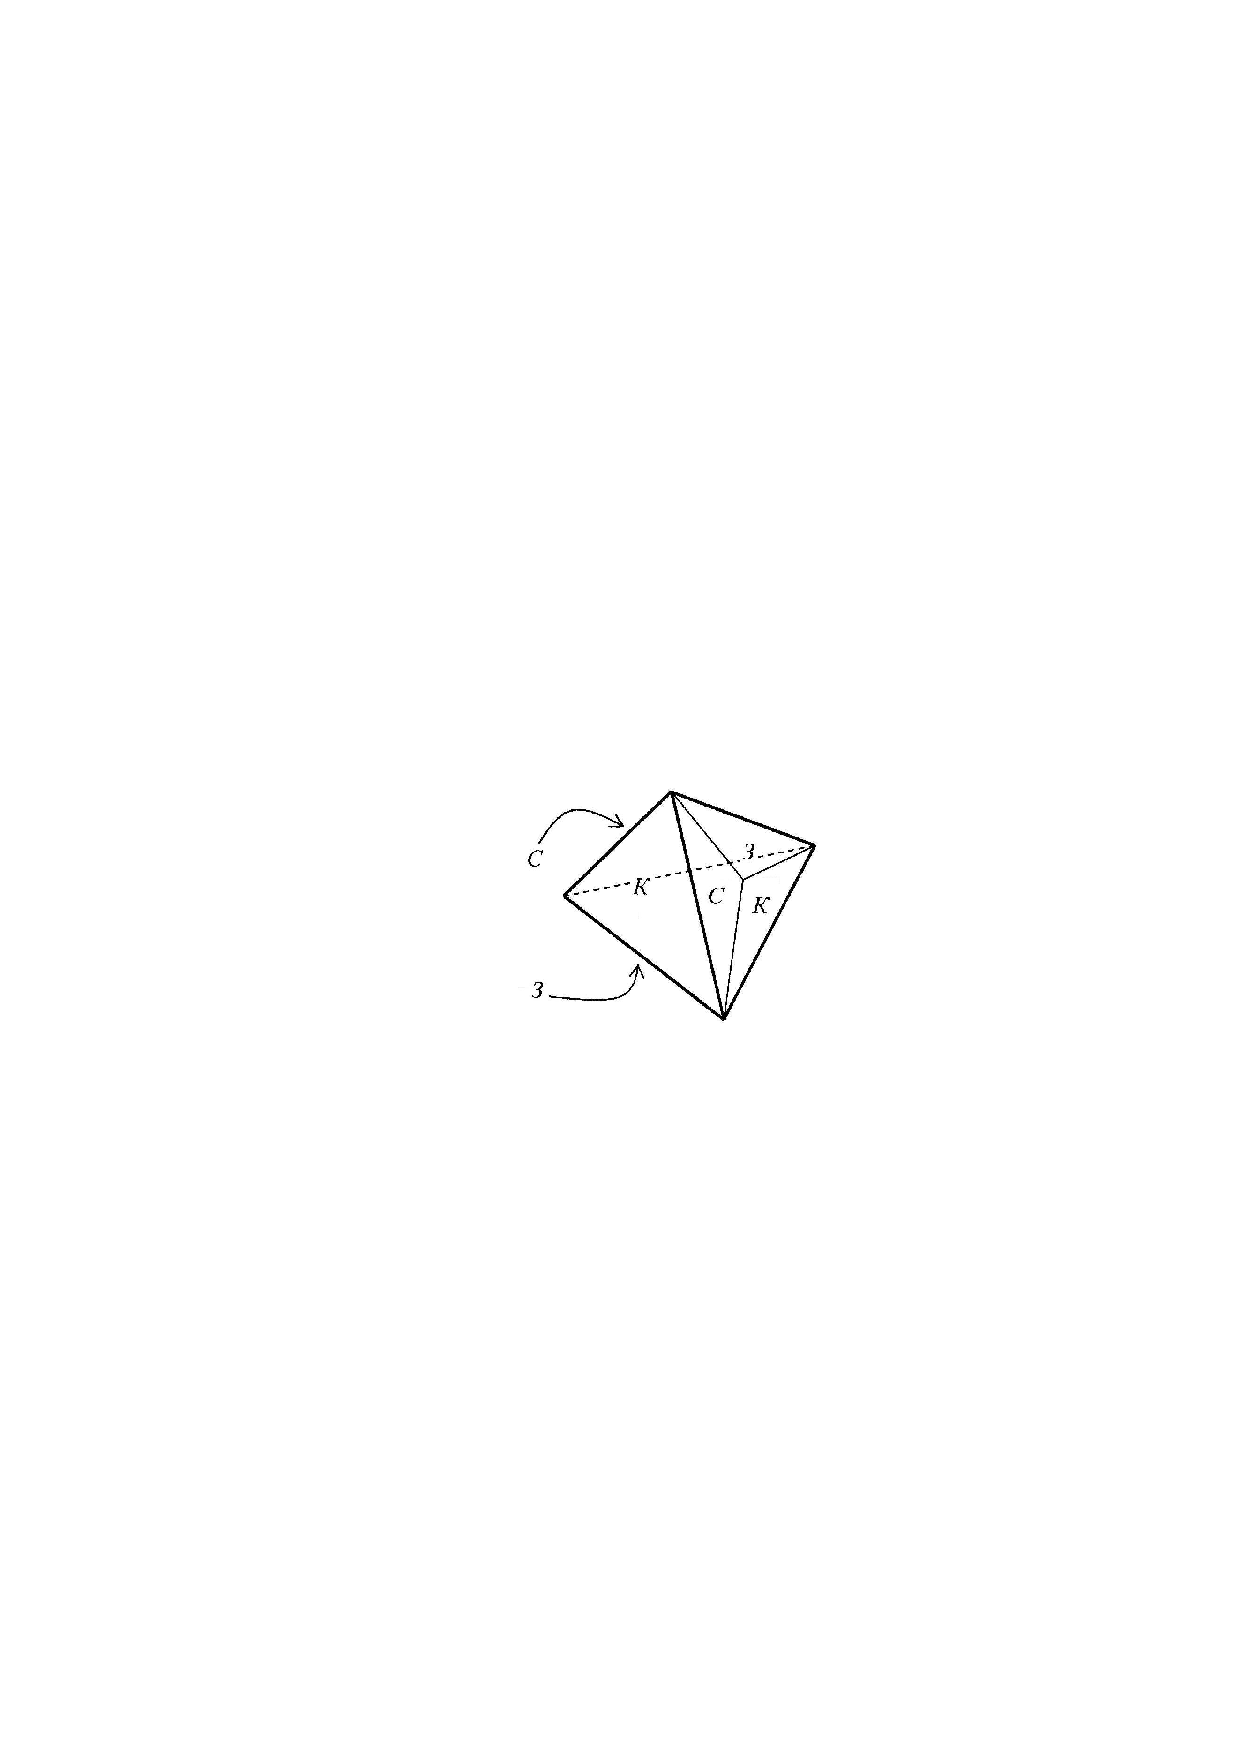
\includegraphics[width=0.5\textwidth]{pic/pic6.pdf}
	\caption{Тетраэдр Бернштейна}
	\label{pic:6}
\end{figure}

\begin{example}[Тетраэдр Бернштейна\footnote{Сергей Натанович Берншейн (1880 — 1968), советский математик.}]
\label{ex:5.5}

Рассмотрим правильный тетраэдр, три грани которого окрашены в эти синий, зелёный, и красный цвет, см. рис. \ref{pic:6},
а четвёртая грань разделена на три треугольника, и эти треугольники окрашены в те же три цвета. Обозначим через $B$, $G$ и $R$ события означающие выпадение снизу грани, содержащей соответственно синий (blue), зелёный
(green), и красный (red) цвета.
Легко видеть, что каждый цвет нарисован на двух из четырёх граней
поэтому $\P(B) = \P(G) = \P(R) = 1/2$. Также легко видеть, что появление
любой пары из них имеет вероятности $\P(B\cap G) = \P(G\cap R) = \P(B\cap R) = 1/4$.
Т.о., для каждой пары из этих событий формула определения \ref{def:5.1} выполнена, и
следовательно события попарно независимы.

Теперь проверим независимость событий $B, G$ и $R$ в совокупности. Легко
видеть, что вероятность $\P(B \cap  G \cap  R)$ выпадения трёхцветной грани равна
1/4. Это левая часть равенства определения \ref{def:5.3}. Правая часть равна $\P(B) \cdot \P(G) \cdot
\P(R) = 1/8$. Т.е. равенство определяемое леммой \ref{lemma:5.2} не выполнено, значит события $B, G$
и $R$ зависимы в совокупности.
\end{example}

% \end{theorem}

